\section{The Software Out-of-Order Processor}
\label{sec:soop}

There are two major challenges in implementing an efficient task
scheduler for Legion:
\begin{itemize}
\item  For correctness, Legion must guarantee that every pair of {\em dependent} tasks is serialized in the correct order.

\item For performance, Legion must hide the extremely long latencies associated
  with machines that have both distributed memory and many levels of
  memory hierarchy.
\end{itemize}
Our scheduler uses three techniques to achieve both correctness and high performance:
\begin{itemize}
\item Subtasks enjoy an isolation property that allows Legion
to avoid comparing all pairs of tasks for dependences.
Specifically, the only tasks that need to be checked for dependences 
are the immediate subtasks of a common
parent task (see Section~\ref{sec:exec}).

\item Legion uses a {\em deferred execution model} that decouples the issuing
of operations from when operations are performed.  Issued operations wait for other operations on
which they are dependent to complete before executing.  For example, Legion may issue a copy
operation to move the results of a task $a$ to the place where a task $b$ will take the copied data as
an argument.  Tasks $a$ and $b$ and the copy can all be issued, but the copy will not start until
task $a$ completes and task $b$ will not start until the copy completes.

\item Legion uses a {\em  software out-of-order processor}, or SOOP, to schedule tasks.  The SOOP 
is distributed and concurrent, and also extracts nested parallelism from subtasks.
\end{itemize}

During execution of a Legion program, each processor runs its own instance of the Legion SOOP.
A processor's SOOP is the Legion runtime system for that processor and handles all requests
for Legion services from tasks executing on the processor.
Legion's SOOP has a five stage pipeline that  separates the management of system resources from actual
task execution.  The five stages are: dependence analysis (Section~\ref{sec:dep}),
distribution (Section~\ref{sec:dist}),
mapping (Section~\ref{sec:map}),
execution (Section~\ref{sec:exec}),
and clean-up (Section~\ref{sec:clean}).
We discuss each in turn.

\usetikzlibrary{calc}
\begin{figure}[t]
  \centering
  \subfigure[mapping of $cnc_0$ task]{
    \label{sfig:mapping_fig:cnc}
    \begin{tikzpicture}[scale=0.8]
      \partitiontree
      \node(cnc_p0)[very thick,draw,fill=white] at (0.45,0.30) {\tiny $cnc_0$};
      \node(cnc_g0)[very thick,draw,fill=white] at (5.45,0.30) {\tiny $cnc_0$};
      \node(def_top)[very thin,draw,fill=white] at (3.3,4.35) {\tiny ~~---~~};
      \draw[very thick] ($ (top.south)!.5!(ptp.center) $) circle (2pt);
      \draw[very thick] ($ (pvsf.north)!.5!(ptf.center) $) circle (2pt);
      \draw[very thick] ($ (pvsf.250)!.5!(ppp.center) $) circle (2pt);
      \draw[very thick] ($ (p0.north)!.5!(pp0.center) $) circle (2pt);
      \draw[very thick] ($ (pvst.north)!.5!(ptt.center) $) circle (2pt);
      \draw[very thick] ($ (pvst.310)!.5!(pgp.center) $) circle (2pt);
      \draw[very thick] ($ (g0.north)!.5!(pg0.center) $) circle (2pt);
      \draw[very thick,->] (def_top) to [bend right=45] (cnc_p0);
      \draw[very thick,->] (def_top) to [bend left=45] (cnc_g0);
    \end{tikzpicture}
  }
  \subfigure[mapping of $dc_0$ task]{
    \label{sfig:mapping_fig:dc}
    \begin{tikzpicture}[scale=0.8]
      \partitiontree
      %\node(cnc_p0)[very thick,draw,fill=white] at (0.45,0.30) {\tiny $\begin{array}{c}\cancel{cnc_0} \\ dc_0\end{array}$};
      \node(dc_p0)[very thick,draw,fill=white] at (0.45,0.30) 
{\tiny
$\begin{array}{@{}c@{}}
\cancel{cnc_0} \\
dc_0
\end{array}$};
      \node(cnc_p1)[very thin,draw,fill=white] at (1.25,0.30) {\tiny $cnc_1$};
      \node(cnc_pn)[very thin,draw,fill=white] at (2.25,0.30) {\tiny $cnc_{n-1}$};
      \node(cnc_g0)[very thin,draw,fill=white] at (5.45,0.30) {\tiny $cnc_0$};
      \node(dc_g0)[very thick,draw,fill=white] at (5.45,0.75) {\tiny $dc_0$};
      \draw[very thick,->] (cnc_g0.west) to [bend left=70] (dc_g0.west);
      \draw[very thick] ($ (cnc_g0.center) - (0.25,0.25) $) -- ++(0.5,0.5);
      \draw[very thick] ($ (cnc_g0.center) - (0.25,-0.25) $) -- ++(0.5,-0.5);
      \node(cnc_g1)[very thin,draw,fill=white] at (6.25,0.30) {\tiny $cnc_1$};
      \node(cnc_gn)[very thin,draw,fill=white] at (7.25,0.30) {\tiny $cnc_{n-1}$};
      \node(def_top)[very thin,draw,fill=white] at (3.3,4.35) {\tiny ~~---~~};
      \draw[very thin] ($ (top.south)!.5!(ptp.center) $) circle (2pt);
      \draw[very thin] ($ (pvsf.north)!.5!(ptf.center) $) circle (2pt);
      \draw[very thin] ($ (pvsf.250)!.5!(ppp.center) $) circle (2pt);
      \draw[very thin] ($ (p0.north)!.5!(pp0.center) $) circle (2pt);
      \draw[very thin] ($ (p1.north)!.5!(pp1.center) $) circle (2pt);
      \draw[very thin] ($ (pn.north)!.5!(ppn.center) $) circle (2pt);
      \draw[very thin] ($ (pvst.north)!.5!(ptt.center) $) circle (2pt);
      \draw[very thin] ($ (pvst.310)!.5!(pgp.center) $) circle (2pt);
      \draw[very thin] ($ (g0.north)!.5!(pg0.center) $) circle (2pt);
      \draw[very thin] ($ (g1.north)!.5!(pg1.center) $) circle (2pt);
      \draw[very thin] ($ (gn.north)!.5!(pgn.center) $) circle (2pt);
    \end{tikzpicture}
  }
  \subfigure[mapping of $volt_0$ task]{
    \label{sfig:mapping_fig:volt}
    \begin{tikzpicture}[scale=0.8]
      \partitiontree
      \node(dc_p0)[very thin,draw,fill=white] at (0.45,0.30) {\tiny $dc_0$};
      \node(dc_p1)[very thin,draw,fill=white] at (1.25,0.30) {\tiny $dc_1$};
      \node(dc_pn)[very thin,draw,fill=white] at (2.25,0.30) {\tiny $dc_{n-1}$};
      \node(dc_g0)[very thin,draw,fill=white] at (5.45,0.30) {\tiny $dc_0$};
      \node(volt_p0)[very thick,draw,fill=white] at (0.45,0.75) {\tiny $volt_0$};
      \draw[very thick,->] (dc_p0.west) to [bend left=70] (volt_p0.west);
      \draw[very thick] ($ (dc_p0.center) - (0.25,0.25) $) -- ++(0.5,0.5);
      \draw[very thick] ($ (dc_p0.center) - (0.25,-0.25) $) -- ++(0.5,-0.5);
      \draw[very thick] ($ (dc_g0.center) - (0.25,0.25) $) -- ++(0.5,0.5);
      \draw[very thick] ($ (dc_g0.center) - (0.25,-0.25) $) -- ++(0.5,-0.5);
      \node(dc_g0)[very thin,draw,fill=white] at (5.45,0.30) {\tiny $dc_0$};
      \node(dc_g1)[very thin,draw,fill=white] at (6.25,0.30) {\tiny $dc_1$};
      \node(dc_gn)[very thin,draw,fill=white] at (7.25,0.30) {\tiny $dc_{n-1}$};
      \draw[very thick] ($ (dc_g0.center) - (0.25,0.25) $) -- ++(0.5,0.5);
      \draw[very thick] ($ (dc_g0.center) - (0.25,-0.25) $) -- ++(0.5,-0.5);
      \draw[very thick] ($ (dc_g1.center) - (0.25,0.25) $) -- ++(0.5,0.5);
      \draw[very thick] ($ (dc_g1.center) - (0.25,-0.25) $) -- ++(0.5,-0.5);
      \draw[very thick] ($ (dc_gn.center) - (0.25,0.25) $) -- ++(0.5,0.5);
      \draw[very thick] ($ (dc_gn.center) - (0.25,-0.25) $) -- ++(0.5,-0.5);
      \node(def_top)[very thin,draw,fill=white] at (3.3,4.35) {\tiny ~~---~~};
      \draw[very thin] ($ (top.south)!.5!(ptp.center) $) circle (2pt);
      \draw[very thin] ($ (pvsf.north)!.5!(ptf.center) $) circle (2pt);
      \draw[very thin] ($ (pvsf.250)!.5!(ppp.center) $) circle (2pt);
      \draw[very thin] ($ (p0.north)!.5!(pp0.center) $) circle (2pt);
      \draw[very thin] ($ (p1.north)!.5!(pp1.center) $) circle (2pt);
      \draw[very thin] ($ (pn.north)!.5!(ppn.center) $) circle (2pt);
      \draw[very thin] ($ (pvst.north)!.5!(ptt.center) $) circle (2pt);
      \draw[very thin] ($ (pvst.310)!.5!(pgp.center) $) circle (2pt);
      \draw[very thin] ($ (g0.north)!.5!(pg0.center) $) circle (2pt);
      \draw[very thin] ($ (g1.north)!.5!(pg1.center) $) circle (2pt);
      \draw[very thin] ($ (gn.north)!.5!(pgn.center) $) circle (2pt);
      \draw[very thick] ($ (g0.north)!.5!(pg0.center) - (0.1,0.1) $) -- ++(0.2,0.2);
      \draw[very thick] ($ (g0.north)!.5!(pg0.center) - (0.1,-0.1) $) -- ++(0.2,-0.2);
      \draw[very thick] ($ (g1.north)!.5!(pg1.center) - (0.1,0.1) $) -- ++(0.2,0.2);
      \draw[very thick] ($ (g1.north)!.5!(pg1.center) - (0.1,-0.1) $) -- ++(0.2,-0.2);
      \draw[very thick] ($ (gn.north)!.5!(pgn.center) - (0.1,0.1) $) -- ++(0.2,0.2);
      \draw[very thick] ($ (gn.north)!.5!(pgn.center) - (0.1,-0.1) $) -- ++(0.2,-0.2);
      \draw[very thick] ($ (pvst.310)!.5!(pgp.center) - (0.1,0.1) $) -- ++(0.2,0.2);
      \draw[very thick] ($ (pvst.310)!.5!(pgp.center) - (0.1,-0.1) $) -- ++(0.2,-0.2);
      \draw[very thick] ($ (pvst.230)!.5!(psp.center) $) circle (2pt);
      \draw[very thick] ($ (s0.north)!.5!(ps0.center) $) circle (2pt);
      \node(def_pvst)[very thick,draw,fill=white] at (5.3,2.75) {\tiny ~~---~~};
      \draw[very thick,->] (dc_g0.north) to [bend right=30] (def_pvst.270);
      \draw[very thick,->] (dc_g1.north) to [bend right=30] (def_pvst.315);
      \draw[very thick,->] (dc_gn.north) to [bend right=30] (def_pvst.0);
      \node(volt_s0)[very thick,draw,fill=white] at (3.2,0.30) {\tiny $volt_0$};
      \draw[very thick,->] (def_pvst.190) to [bend right=40] (volt_s0.130);
    \end{tikzpicture}
  }
  \label{fig:mapping_fig}
  \caption{Mapping of tasks in region tree}
\end{figure}




\subsection{Depedence Analysis}
\label{sec:dep}


When a Legion task runs, it may spawn new subtasks to be executed.
Each subtask is {\em registered} with the local SOOP in sequential execution
order, which records the subtask's logical region arguments and associated privileges and coherence properties.  If two subtasks work on indepedent data Legion can schedule
them to out of order, in parallel.  Thus, the first stage in the
execution of a task is dependence analysis between tasks.

Conceptually, detecting dependences between a newly registered task $t$ and a previous task 
$t'$ requires comparing the two sets of logical regions accessed.  For each logical region used by
$t'$ that may overlap with a logical region used by $t$, the privileges
and coherence modes are compared to determine whether a dependence exists.  If
both regions need only read privileges there is never a dependence, but if either
task needs write or reduction privileges, the coherence modes are compared:
{\small
\begin{tabular}{c|cccc}
             & Exclusive & Atomic   & Simultaneous & Relaxed \\
\midrule
Exclusive    & Dep & Dep & Dep & Dep \\ 
Atomic       & Dep & Same & Cont & Cont \\
Simultaneous & Dep & Cont & Same & None \\
Relaxed      & Dep & Cont & None & None \\
\end{tabular}
}

An {\tt Dep} entry indicates dependence while {\tt None}
indicates independence.  A {\tt Same} entry is a dependence unless the two tasks
use the same {\em physical region}.  Finally, a {\tt Cont} entry
indicates a dependence unless a single writer is using the
atomic coherence mode.  When a dependence is detected, the new task
waits for the older task to complete before it begins execution.

The table lists {\em simultaneous} and {\em relaxed} coherence modes
that we have not yet discussed.  Both simultaneous and relaxed
allow other tasks using the region to execute at the same time and differ
only in what data must be observed.  With simultaneous coherence, a task must 
see all updates to the logical region made by other tasks operating on the same region 
simultaneously (i.e., shared memory semantics).  With relaxed coherence, 
a task may or may not observe updates to the logical region by other tasks executing at
the same time.

% *****  isolation, efficient data structure ******

To detect dependencies efficiently, the high-level runtime maintains a
local region forest (recall Section~\ref{sec:exec}) for each task.  The
root regions are the task's region arguments, and the forest includes
all partitions and subregions created within the task.  To perform
dependence detection on a region $r$, the runtime first finds a root
region $r'$ such that $r \rleq r'$.  The runtime then walks the region
forest from $r'$ to $r$.  Each region $r''$ on the path contains a
list $L$ of registered tasks using $r''$, and potential dependencies
are discovered by comparing privileges and coherence modes with the
tasks in $L$.

The runtime next checks if a partition of $r''$ is {\em open}.  An
open partition indicates that there are active tasks using subregions
of $r''$.  No more than one partition of a node can be open
at any time.  If the open partition is is along the path to $r$,
traversal continues.  If the open partition lies along another
path the runtime must {\em close} the currently active partition because it cannot guarantee
disjointness with the region the new task wishes to access.  To close a
partition, the runtime finds all active tasks in that
subtree and considers them all dependencies for the new task.
With the previously active partition closed, the runtime can
then open the desired partition and traverse further down the tree as
needed.

When the runtime traverses an open partition, its behavior depends on the kind
of partition being traversed.  If the partition is disjoint, no other subregion
can overlap with the target region, so the state of other subregions is
ignored.  However, if the partition is not disjoint, any
of subregion could overlap with the desired subregion, so
the runtime must close all open subregions (recording new dependencies
as it does so) before continuing the traversal.

After the runtime reaches the target logical region, it performs dependence
checks against any active tasks listed for that region.  If a dependence is
discovered, it is added to the current task's dependence list.  It can then
be removed from the region tree's active task list, as the current task (which
will be pushed onto the active task list) {\em dominates} the previous task.
In a case where the new task has dependencies with all existing active tasks
for the target node, that whole list is replaced by a single entry for the
new task.


\subsection{Distribution}
\label{sec:dist}

\subsection{Mapping}
\label{sec:map}

\subsection{Execution}
\label{sec:exec}

\begin{figure}
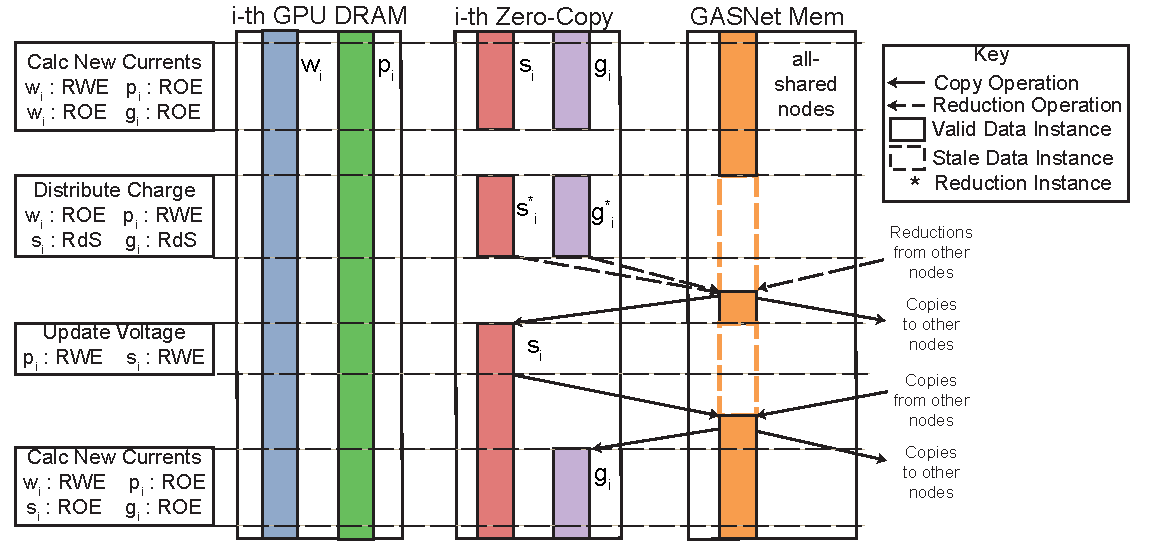
\includegraphics[scale=0.48]{figs/CircuitMem.pdf}
\caption{Tasks and data for the circuit simulation on a cluster of GPUs.}
\end{figure}

\subsection{Clean-Up}
\label{sec:clean}

